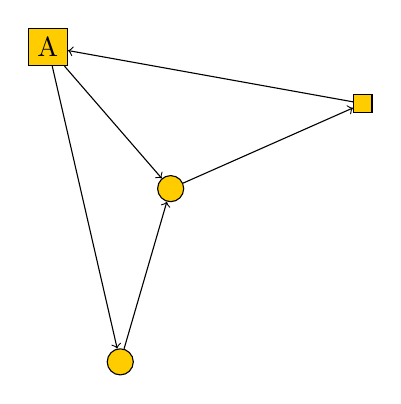
\begin{tikzpicture}[rotate=0,scale=4]
%Define all colors here.

\definecolor{n0fill}{RGB}{255,204,0}
\definecolor{n0text}{RGB}{0,0,0}
\definecolor{n0draw}{RGB}{0,0,0}
\node(n0) at (1.0,-0.18) [rectangle, draw=n0draw, fill=n0fill, text=n0text] {};

\definecolor{n1fill}{RGB}{255,204,0}
\definecolor{n1text}{RGB}{0,0,0}
\definecolor{n1draw}{RGB}{0,0,0}
\node(n1) at (0.23,-1.0) [circle, draw=n1draw, fill=n1fill, text=n1text] {};

\definecolor{n2fill}{RGB}{255,204,0}
\definecolor{n2text}{RGB}{0,0,0}
\definecolor{n2draw}{RGB}{0,0,0}
\node(A) at (0.0,-0.0) [rectangle, draw=n2draw, fill=n2fill, text=n2text] {A};

\definecolor{n3fill}{RGB}{255,204,0}
\definecolor{n3text}{RGB}{0,0,0}
\definecolor{n3draw}{RGB}{0,0,0}
\node(n3) at (0.39,-0.45) [circle, draw=n3draw, fill=n3fill, text=n3text] {};

\draw[->] (A) edge (n1);
\draw[->] (n1) edge (n3);
\draw[->] (n3) edge (n0);
\draw[->] (n0) edge (A);
\draw[->] (A) edge (n3);
\end{tikzpicture}
